\section{Walks, trails, paths, and cycles}\label{sec:walks}

This section answers question (Q3), the definition of a path between $n_i$
and $n_j$, in the order in which the textbook builds the concepts
\cite[pp.~21--23]{petrosyan2015graphs}: walk, closed walk, trail, path,
cycle, distance. Each concept is a small change to the one before it. The
examples use the graph $H$ on five vertices with edges $n_1n_2$, $n_2n_3$,
$n_1n_3$, $n_3n_4$, $n_4n_5$ (\cref{fig:graphs}, middle), which is this
note's own example, not the textbook's; the classification of every
sequence below was checked by script (\cref{app:repro}).

Only walks and paths (\cref{def:walk,def:path,def:pathbetween}) and the
lemmas on them are needed for (Q1) to (Q3). Trails are included because the
textbook uses the word ``path'' for them and its definition of connected
rests on that word; cycles and distance are included to keep the textbook's
order, and distance is used in \cref{cor:dist}.

\begin{figure}[ht]
\centering
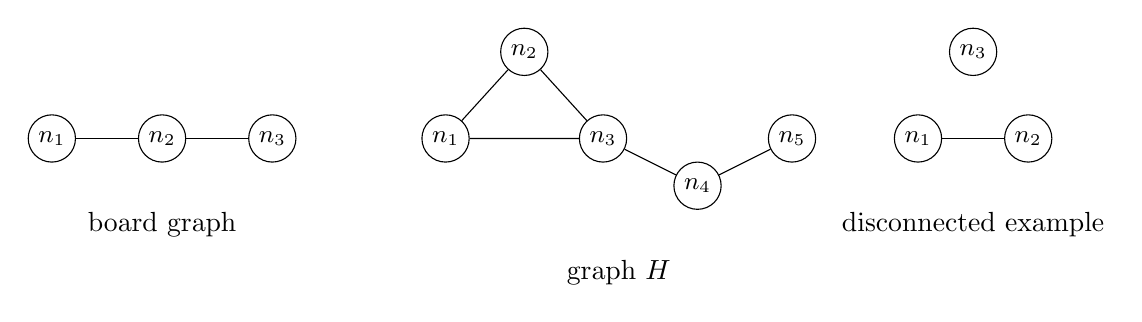
\begin{tikzpicture}[v/.style={circle,draw,inner sep=1.2pt,minimum size=6mm,font=\small},scale=1]
% board graph
\begin{scope}
\node[v] (a1) at (0,0) {$n_1$};
\node[v] (a2) at (1.4,0) {$n_2$};
\node[v] (a3) at (2.8,0) {$n_3$};
\draw (a1)--(a2)--(a3);
\node at (1.4,-1.1) {board graph};
\end{scope}
% graph H
\begin{scope}[xshift=5cm]
\node[v] (b1) at (0,0) {$n_1$};
\node[v] (b2) at (1,1.1) {$n_2$};
\node[v] (b3) at (2,0) {$n_3$};
\node[v] (b4) at (3.2,-0.6) {$n_4$};
\node[v] (b5) at (4.4,0) {$n_5$};
\draw (b1)--(b2)--(b3)--(b1);
\draw (b3)--(b4)--(b5);
\node at (2.2,-1.7) {graph $H$};
\end{scope}
% disconnected example
\begin{scope}[xshift=11cm]
\node[v] (c1) at (0,0) {$n_1$};
\node[v] (c2) at (1.4,0) {$n_2$};
\node[v] (c3) at (0.7,1.1) {$n_3$};
\draw (c1)--(c2);
\node at (0.7,-1.1) {disconnected example};
\end{scope}
\end{tikzpicture}
\caption{The graphs used in the examples. Left: the board graph, with
edges $n_1n_2$ and $n_2n_3$ and the adjacency matrix of the board
(Convention~\ref{conv:drawing}). Middle: the graph $H$ of this section, with edges $n_1n_2$, $n_2n_3$,
$n_1n_3$, $n_3n_4$, $n_4n_5$.
Right: one edge and an isolated vertex, the disconnected example of
\cref{sec:connectivity}.}\label{fig:graphs}
\end{figure}

\paragraph{Notation.} A \emph{$(u,v)$-walk} is a walk from $u$ to $v$.
In examples, a sequence of vertices such as $n_1n_2n_3$ is written
without commas.

\subsection{The definitions}

\plainwords{} A frog sits on an island. It hops over a bridge to a
next-door island, then hops again. The list of islands it visits is a
trip. A trip may land on an island again. It may use a bridge again. The
number of hops is how long the trip is. A frog that does not hop at all
makes a trip with no hops.

\begin{definition}[Walk; textbook Definition~1.2.10]\label{def:walk}
A \emph{walk from $u_0$ to $u_k$} is a sequence of vertices
$u_0u_1\cdots u_k$ in which each vertex is adjacent to the one before it;
its \emph{length} is $k$, the number of edges used. Formally, the textbook
defines it as a sequence $u_0,e_1,u_1,\dots,e_k,u_k$ of vertices and edges
with $e_t=u_{t-1}u_t$ for $1\le t\le k$
\cite[Definition~1.2.10, p.~21]{petrosyan2015graphs}; in a simple graph the
edges are fixed by the vertices, so the vertex sequence says the same. This
note allows $k=0$ (Convention~\ref{conv:length}), which the textbook's
definition does not state in words.
\end{definition}

\begin{remark}
Vertices and edges may repeat, and the length counts each edge as often as
it is used \cite[p.~22]{petrosyan2015graphs}. A single vertex $u$ is a walk
of length 0 from $u$ to $u$ (Convention~\ref{conv:length}).
\end{remark}
\begin{example}
In $H$, the sequence $n_1n_2n_3n_4n_3n_1$ is a walk of length $5$.
\end{example}
\begin{nonexample}
In $H$, the sequence $n_1n_4$ is not a walk, because $n_1n_4$ is not an
edge.
\end{nonexample}

\plainwords{} A round trip ends on the island where it began.

\begin{definition}[Closed walk; textbook Definition~1.2.11]\label{def:closed}
A walk $u_0\cdots u_k$ is \emph{closed} if $u_0=u_k$
\cite[Definition~1.2.11, p.~22]{petrosyan2015graphs}.
\end{definition}

\begin{remark}
A walk of length 0 is closed, and so is a walk that goes along one edge
and straight back.
\end{remark}
\begin{example}
In $H$, the walk $n_1n_2n_1$ is closed.
\end{example}
\begin{nonexample}
In $H$, the walk $n_1n_2n_3$ is not closed.
\end{nonexample}

\plainwords{} A fresh-bridge trip never uses the same bridge twice. It may
land on an island again.

\begin{definition}[Trail; textbook Definition~1.2.12, where it is called ``path'']\label{def:trail}
A walk is a \emph{trail} if its edges $u_0u_1,\dots,u_{k-1}u_k$ are
pairwise distinct. Its length is its number of edges
\cite[Definition~1.2.12, p.~22]{petrosyan2015graphs}.
\end{definition}

\begin{remark}
The textbook's word for a trail is ``path'' (Convention~\ref{conv:path}),
which is not what this note means by ``path''. In a trail vertices may
repeat but edges may not. The English word ``trail'' for this notion is
used by Grinberg \cite[Definition~3.4.5, p.~101]{grinberg2025graph}; it is
this note's choice for the textbook's concept, because the course's word
for it was not reported.
\end{remark}
\begin{example}
In $H$, the walk $n_3n_1n_2n_3n_4$ is a trail: its edges $n_3n_1$,
$n_1n_2$, $n_2n_3$, $n_3n_4$ are distinct, although $n_3$ occurs twice.
\end{example}
\begin{nonexample}
In $H$, the walk $n_1n_2n_1n_3$ is not a trail, because it uses the edge
$n_1n_2$ twice.
\end{nonexample}

\plainwords{} A fresh-island trip never lands on the same island twice.

\begin{definition}[Path; textbook Definition~1.2.13, the ``simple path'']\label{def:path}
A walk is a \emph{path} if its vertices $u_0,\dots,u_k$ are pairwise
distinct. This is the textbook's simple path, defined there as a
textbook ``path'' (a trail) with distinct vertices
\cite[Definition~1.2.13, p.~22]{petrosyan2015graphs}; it is the course
convention (Convention~\ref{conv:path}).
\end{definition}

\begin{remark}
Every path is a trail, because distinct vertices force distinct edges
(\cref{lem:distinct}); every trail is a walk; the converses fail. This is
why the definition here needs only ``no repeated vertex'', whereas the
textbook states it as a trail with distinct vertices.
\end{remark}
\begin{example}
In $H$, the walk $n_1n_3n_4n_5$ is a path of length $3$, and so is
$n_1n_2n_3n_4n_5$, of length $4$.
\end{example}
\begin{nonexample}
In $H$, the trail $n_3n_1n_2n_3n_4$ is not a path, because $n_3$ occurs
twice. The walk $n_1n_2n_1$ is not a path either.
\end{nonexample}

\plainwords{} Pick two islands. Sometimes the frog can get from the first to the
second. If it lands on no island twice, that is a fresh-island trip between
them. A frog that stays put makes such a trip from an island to itself.

\begin{definition}[Path between $n_i$ and $n_j$; the answer to (Q3)]\label{def:pathbetween}
Let $n_i,n_j\in V$. A \emph{path between $n_i$ and $n_j$} (also a path
\emph{from $n_i$ to $n_j$}) is a sequence $u_0,u_1,\dots,u_k$ with
$k\ge 0$, $u_0=n_i$, $u_k=n_j$, such that $u_{t-1}$ and $u_t$ are adjacent
for $1\le t\le k$ and $u_0,\dots,u_k$ are pairwise distinct. Its length is
$k$. This is \cref{def:path} with the ends fixed, that is, the
textbook's Definition~1.2.13 with ends $n_i$ and $n_j$.
\end{definition}

\begin{remark}
If $i\ne j$, such a path has at least one edge. If $i=j$, the only path is
the single vertex $(n_i)$ of length 0, because $u_0=u_k$ with $k\ge 1$
would repeat a vertex. Two vertices may be joined by several paths of
different lengths.
\end{remark}
\begin{example}
In the board graph the only path from $n_1$ to $n_3$ is $n_1n_2n_3$, of
length $2$. In $H$ there are two paths from $n_1$ to $n_4$: $n_1n_3n_4$
and $n_1n_2n_3n_4$.
\end{example}
\begin{nonexample}
In the board graph, $n_1n_2n_1n_2n_3$ is a walk from $n_1$ to $n_3$ but not
a path, because it repeats $n_1$. And $n_1n_2n_1$ is not a path from $n_1$
to $n_1$.
\end{nonexample}

\plainwords{} Some round trips never use a bridge twice. If such a round trip
also lands twice on no island except the first, we call it a ring trip. A
ring trip needs at least three bridges.

\begin{definition}[Closed trail and cycle; textbook Definitions 1.2.14 and 1.2.15]\label{def:cycle}
A \emph{closed trail} is a closed walk that is a trail. The textbook calls
it a ``closed path or cycle'' \cite[Definition~1.2.14,
p.~22]{petrosyan2015graphs}. A \emph{cycle} is a closed trail of positive
length whose only repeated vertices are its first and last; this is the
textbook's simple cycle \cite[Definition~1.2.15, p.~22]{petrosyan2015graphs}
and the English ``cycle''. The word ``cycle'' is used only in this sense.
\end{definition}

\begin{remark}
In a simple graph a cycle has length at least $3$. Length $1$ would need an
edge from a vertex to itself. Length $2$ would be $w_0w_1w_0$, which uses
the edge $w_0w_1$ twice and is not a trail. The textbook's $C_n$ has
$n\ge 3$ \cite[p.~22]{petrosyan2015graphs}. A closed trail need not be a
cycle: in the graph with edges $n_1n_2$, $n_2n_3$, $n_1n_3$, $n_1n_4$,
$n_4n_5$, $n_1n_5$ (two triangles sharing $n_1$), the sequence
$n_1n_2n_3n_1n_4n_5n_1$ is a closed trail of length $6$ that repeats $n_1$
in the middle.
\end{remark}
\begin{example}
In $H$, the walk $n_1n_2n_3n_1$ is a cycle of length $3$.
\end{example}
\begin{nonexample}
In $H$, the walk $n_1n_2n_1$ is a closed walk but not a closed trail. The
board graph has no cycle at all.
\end{nonexample}

\plainwords{} The fewest hops between two islands is how far apart they
are. If the frog can never get from one to the other, we say they are
infinitely far apart.

\begin{definition}[Distance; textbook Definition~1.2.16]\label{def:distance}
The \emph{distance} $d(u,v)$ is the length of a shortest $(u,v)$-trail if
there is one, and $\infty$ otherwise
\cite[Definition~1.2.16, pp.~22--23]{petrosyan2015graphs}. (The textbook
words this with its own ``path'', that is, trail.)
\end{definition}

\begin{remark}
The textbook measures distance by shortest trails. \Cref{prop:distance}
shows that shortest walks and shortest paths give the same number, so this
note may say ``shortest path'' without changing the textbook's value.
\end{remark}
\begin{example}
In the board graph, $d(n_1,n_3)=2$ and $d(n_1,n_1)=0$.
\end{example}
\begin{nonexample}
Add an isolated vertex $n_4$ to the board graph. Then $d(n_1,n_4)=\infty$,
not $0$ or $3$.
\end{nonexample}

\begin{table}[ht]
\centering
\begin{tabular}{@{}p{3.6cm}p{2.5cm}p{3.4cm}p{2.2cm}p{1.5cm}@{}}
\toprule
Concept & This note (course) & Textbook's word & English & Textbook number \\
\midrule
walk, length $k\ge 0$ & walk & walk & walk & 1.2.10 \\
walk with first vertex equal to last & closed walk & closed walk & closed walk & 1.2.11 \\
walk with no repeated edge & trail & ``path'' & trail & 1.2.12 \\
walk with no repeated vertex & path & ``simple path'' & path & 1.2.13 \\
closed trail & closed trail & ``closed path or cycle'' & closed trail & 1.2.14 \\
closed trail, only first and last vertex repeat & cycle & ``simple cycle'' & cycle & 1.2.15 \\
least length of such a walk & distance & distance & distance & 1.2.16 \\
\bottomrule
\end{tabular}
\caption{Three naming conventions for the same concepts. The textbook
column is from \cite[pp.~21--23]{petrosyan2015graphs}. The English column
is the usage of Grinberg \cite[Definitions~2.9.1(c), 2.10.1(b),
3.4.5]{grinberg2025graph} and of Bai, who defines a path as a walk where no
vertex is repeated \cite[p.~1]{bai2025adjacency}; it is the usage of those
two sources, not a survey of English books. The word ``trail'' in the
middle column is this note's choice (Convention~\ref{conv:path}).}\label{tab:naming}
\end{table}

\subsection{Results about walks and paths}

\plainwords{} A fresh-island trip never lands on an island twice. So it
cannot use the same bridge twice either.

\begin{lemma}[Distinct vertices give distinct edges]\label{lem:distinct}
A walk $u_0\cdots u_k$ whose vertices are pairwise distinct has pairwise
distinct edges. Hence every path is a trail.
\end{lemma}
The textbook's Definition~1.2.13 asks for both properties
\cite[p.~22]{petrosyan2015graphs}; the proof is the note's own.
\begin{proof}
Suppose two edges are equal, $e_s=e_t$ with positions $1\le s<t\le k$,
where $e_s=\{u_{s-1},u_s\}$ and $e_t=\{u_{t-1},u_t\}$. The vertex $u_{s-1}$
is an end of $e_s$, hence an end of $e_t$, so $u_{s-1}=u_{t-1}$ or
$u_{s-1}=u_t$. Because the vertices of the walk are pairwise distinct, two
of them are equal only if they have the same position, so $s-1=t-1$ or
$s-1=t$. Both are impossible, because $s<t$. So no two edges are equal.
\end{proof}

\plainwords{} Take any trip from one island to another. Suppose the frog
lands on some island twice. Cut out all the hops between the two visits.
What is left is still a trip between the same two islands. It has fewer
hops. Keep cutting. In the end the frog lands on no island twice.

\begin{lemma}[Every walk contains a path]\label{lem:cut}
Let $W=u_0\cdots u_k$ be a walk from $u$ to $v$ (equal or not). Then there
is a path from $u$ to $v$ of length at most $k$ whose edges are edges of
$W$.
\end{lemma}
The textbook's Lemma~1.2.1 states this for $u\ne v$, without a bound on
the length, and proves it by induction on the length of the walk
\cite[Lemma~1.2.1, p.~23]{petrosyan2015graphs}. Grinberg's
Corollary~2.9.7 covers $u=v$ and gives the bound
\cite[p.~39]{grinberg2025graph}. The proof below, which allows $k=0$, is the
note's own.
\begin{proof}
By strong induction on $k$: to prove the statement for walks of length $k$,
we may assume it for all shorter walks, of every length from $0$ to
$k-1$. (Ordinary induction would assume it only for length $k-1$; we need
more, because the cut below removes an unknown number of edges.)
\emph{Base case $k=0$.} Then $W=(u)$ has one vertex, which is not repeated,
so $W$ is itself a path of length $0$.
\emph{Inductive case.} Let $k\ge 1$ and assume the statement for all walks
shorter than $k$. If the vertices of $W$ are pairwise distinct, $W$ is a
path of length $k$. Otherwise there are positions $s<t$ with $u_s=u_t$,
the same vertex visited twice. Form $W'=u_0\cdots u_su_{t+1}\cdots u_k$,
that is, delete the part of $W$ between the two visits (if $t=k$, then
$W'=u_0\cdots u_s$). It is a walk, because the only new consecutive pair is
$u_s,u_{t+1}$ and $u_s=u_t$ is adjacent to $u_{t+1}$. It runs from $u$ to
$v$, its edges are edges of $W$, and its length is $k-(t-s)<k$. By the
induction hypothesis $W'$ contains a path from $u$ to $v$ of length at most
$k-(t-s)\le k$. (The example after this proof shows the cut.)
\end{proof}

\begin{example}
In the board graph, cutting the walk $n_1n_2n_1n_2n_3$ at the repeated
vertex $n_1$ leaves the path $n_1n_2n_3$; cutting the closed walk
$n_1n_2n_3n_2n_1$ leaves the path $n_1$ of length $0$.
\end{example}

\plainwords{} A fresh-island trip lands on each island at most once. So it
cannot have as many hops as there are islands. With three islands, it has
at most two hops.

\begin{corollary}[Length bound]\label{cor:bound}
A path in a graph with $N$ vertices has length at most $N-1$. Hence if
some walk joins $u$ to $v$, a path of length at most $N-1$ joins them.
\end{corollary}
\begin{proof}
A path of length $k$ has $k+1$ pairwise distinct vertices among the $N$
vertices of the graph, so $k+1\le N$ \cite[Section~2.9.4,
p.~40]{grinberg2025graph}. The second sentence follows with
\cref{lem:cut}: a walk of any length contains a path, and every path has
length at most $N-1$.
\end{proof}
The bound is attained: the path graph on $N$ vertices has a path of length
$N-1$.

\plainwords{} Suppose some trip joins two islands. Then a fresh-bridge trip
joins them, and a fresh-island trip joins them too. So it does not matter
which kind of trip we ask for.

\begin{proposition}[Walk, trail, and path exist together]\label{prop:together}
For vertices $u$ and $v$ the following are equivalent: (a) a $(u,v)$-walk
exists; (b) a $(u,v)$-trail exists; (c) a $(u,v)$-path exists.
\end{proposition}
Grinberg's Proposition~2.9.10 states the equivalence of walks and paths
only \cite[p.~42]{grinberg2025graph}; the trail case is proved here.
\begin{proof}
(c) implies (b) by \cref{lem:distinct}. (b) implies (a), because a trail
is a walk. (a) implies (c) by \cref{lem:cut}.
\end{proof}
Consequently the textbook's definition of a connected graph, which asks
for a textbook ``path'' (a trail), the board's definition, read with the
course's path, and a definition by walks select the same graphs
(\cref{sec:connectivity}).

\plainwords{} The fewest hops over all trips between two islands is the
same as the fewest hops over all fresh-bridge trips. It is also the same as
the fewest hops over all fresh-island trips.

\begin{proposition}[Distance]\label{prop:distance}
For vertices $u$ and $v$ let $L_w$, $L_t$, $L_p$ be the least length of a
walk, a trail, and a path from $u$ to $v$ (with $\infty$ if none exists).
Then $L_w=L_t=L_p=d(u,v)$.
\end{proposition}
The textbook lists three properties of distance without proof
\cite[p.~23]{petrosyan2015graphs}; the statement here and its proof are the
note's own.
\begin{proof}
Every path is a trail and every trail is a walk (\cref{lem:distinct}), so
$L_w\le L_t\le L_p$. If a walk $W$ of least length $L_w$ exists and
repeated a vertex, the cut in the proof of \cref{lem:cut} would give a
shorter walk, contradicting minimality; so $W$ is a path and
$L_p\le L_w$. The three numbers agree. The textbook's $d(u,v)$ is $L_t$ by
\cref{def:distance}. If no walk exists, all three are $\infty$.
\end{proof}

\begin{remark}
The textbook's three properties of distance then follow from walks
\cite[p.~23]{petrosyan2015graphs}. First, $d(u,v)=0$ exactly when $u=v$,
because a walk of length $0$ ends where it starts (this uses
Convention~\ref{conv:length}). Second, $d(u,v)=d(v,u)$, because reversing a
walk gives a walk of the same length. Third,
$d(u,v)\le d(u,w)+d(w,v)$, because a walk from $u$ to $w$ followed by a
walk from $w$ to $v$ is a walk from $u$ to $v$ whose length is the sum
(trivially true when a distance is $\infty$).
\end{remark}
